% !TeX program = xelatex
% !TeX encoding = UTF-8
\documentclass[10pt, letterpaper]{article}

\usepackage[ignoreheadfoot, top=0.52cm, bottom=0.42cm, left=0.38cm, right=0.38cm, footskip=0.8cm]{geometry}
\usepackage{iftex}
\ifPDFTeX%
  \usepackage[utf8]{inputenc}
  \usepackage{CJKutf8}
\else
  \usepackage[UTF8, fontset=fandol]{ctex}
\fi
\usepackage{titlesec}
\usepackage{tabularx}
\usepackage{array}
\usepackage{graphicx}
\usepackage[dvipsnames]{xcolor}
\definecolor{primaryColor}{RGB}{0, 79, 144}
\usepackage{enumitem}
\usepackage{fontawesome5}
\usepackage{amsmath}
\usepackage[
  pdftitle={Zhang Zhaopeng - Planning and Control CV},
  pdfauthor={Zhang Zhaopeng},
  pdfcreator={LaTeX},
  colorlinks=true,
  urlcolor=primaryColor
]{hyperref}
\usepackage[pscoord]{eso-pic}
\usepackage{calc}
\usepackage{bookmark}
\usepackage{lastpage}
\usepackage{changepage}
\usepackage{paracol}
\usepackage{ifthen}
\usepackage{needspace}
\ifPDFTeX
  \input{glyphtounicode}
  \pdfgentounicode=1
  \usepackage{lmodern}
\fi

\AtBeginEnvironment{adjustwidth}{\partopsep0pt}
\pagestyle{empty}
\setcounter{secnumdepth}{0}
\setlength{\parindent}{0pt}
\setlength{\topskip}{0pt}
\setlength{\columnsep}{0cm}
\linespread{0.92}\selectfont

\titleformat{\section}{\needspace{4\baselineskip}\bfseries\large}{}{0pt}{}[\vspace{1pt}{\color{gray!40}\titlerule}]

\titlespacing{\section}{-1pt}{0.18 cm}{0.10 cm}

\renewcommand\labelitemi{$\circ$}
\newenvironment{highlights}{
  \begin{itemize}[
    topsep=0.02 cm,
    parsep=0pt,
    partopsep=0pt,
    itemsep=0pt,
    leftmargin=0.4 cm + 8pt
  ]
}{
  \end{itemize}
}

\newenvironment{onecolentry}{
  \begin{adjustwidth}{0.2 cm}{0.2 cm}
}{
  \end{adjustwidth}
}

\newenvironment{twocolentry}[2][]{
  \onecolentry
  \def\secondColumn{#2}
  \setcolumnwidth{\fill, 3.5 cm}
  \begin{paracol}{2}
}{
  \switchcolumn\raggedleft\secondColumn
  \end{paracol}
  \endonecolentry
}

\newenvironment{header}{
  \setlength{\topsep}{0pt}\par\kern\topsep\centering\linespread{1.5}
}{
  \par\kern\topsep
}

\newcommand{\placelastupdatedtext}{
  \AddToShipoutPictureFG*{
    \put(
      \LenToUnit{\paperwidth-1.0cm},
      \LenToUnit{\paperheight-0.5cm}
    ){\vtop{{\null}\makebox[0pt][c]{
      \ifPDFTeX%
        \small\color{gray}\textit{Last updated: 2026--08}\hspace{\widthof{Last updated: 2026--08}}
      \else
        \small\color{gray}\textit{最后更新于 2026.08}\hspace{\widthof{最后更新于 2026 年 8 月}}
      \fi
    }}}%
  }%
}

\newcommand{\placecvphoto}{
  \IfFileExists{zhaopeng.png}{
    \AddToShipoutPictureFG*{
      \put(
        \LenToUnit{\paperwidth-2.5cm},
        \LenToUnit{\paperheight-3.0cm}
      ){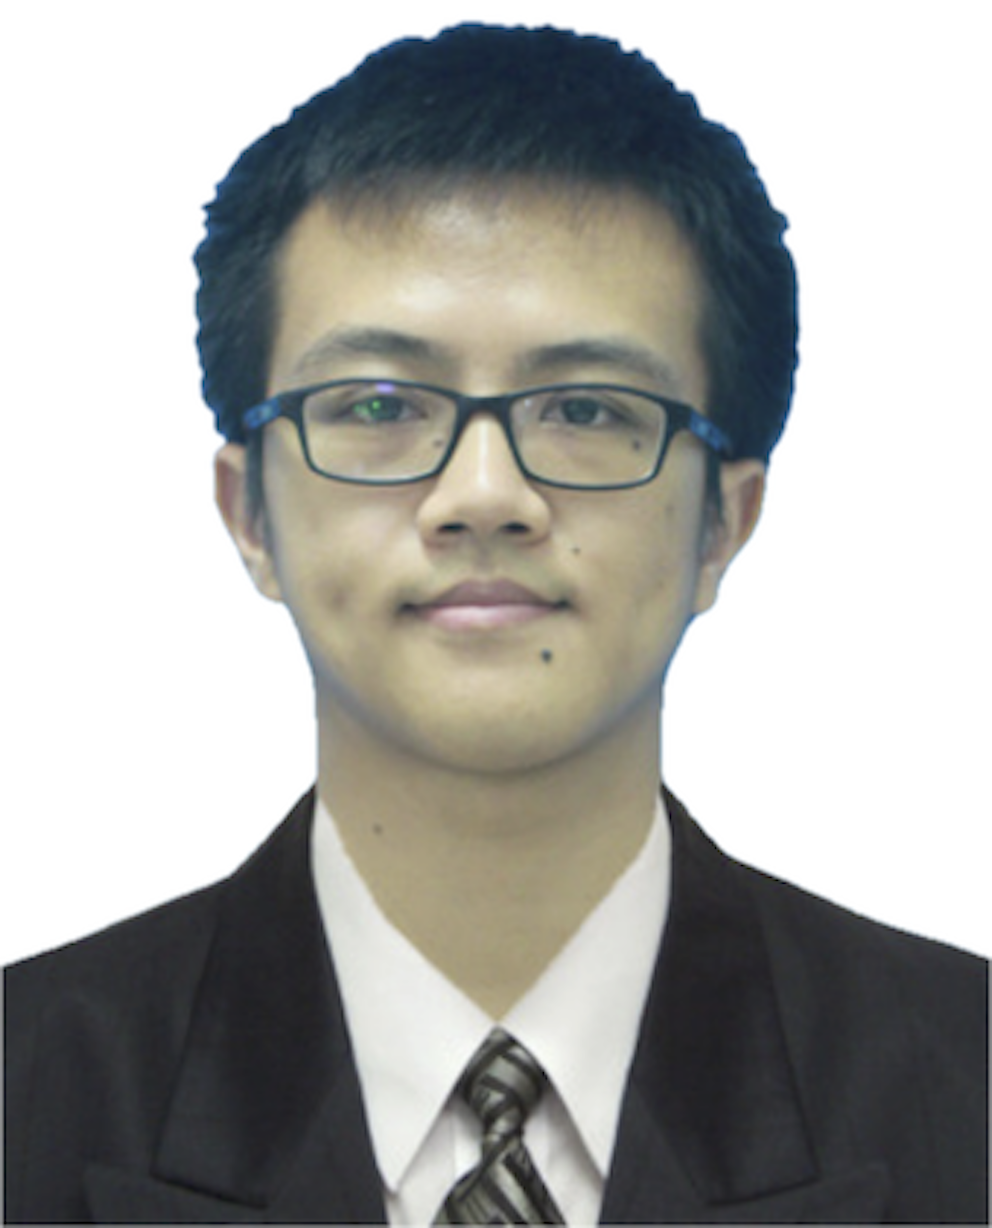
\includegraphics[width=2.2cm]{zhaopeng.png}}
    }%
  }{
    \IfFileExists{CV/Zhaopeng_Zhang.pdf}{
      \AddToShipoutPictureFG*{
        \put(
          \LenToUnit{\paperwidth-2.5cm},
          \LenToUnit{\paperheight-3.0cm}
        ){\includegraphics[width=2.2cm,page=1]{CV/Zhaopeng_Zhang.pdf}}
      }%
    }{}
  }
}

\let\hrefWithoutArrow\href
\renewcommand{\href}[2]{\hrefWithoutArrow{#1}{\ifthenelse{\equal{#2}{}}{ }{#2 }\raisebox{.15ex}{\footnotesize \faExternalLink*}}}

\begin{document}
\ifPDFTeX%
  \begin{CJK*}{UTF8}{gbsn}
\fi
\newcommand{\AND}{\unskip\cleaders\copy\ANDbox\hskip\wd\ANDbox\ignorespaces}
\newsavebox\ANDbox\sbox\ANDbox{}

% \placelastupdatedtext%
\placecvphoto
\begin{header}
  \textbf{\fontsize{20 pt}{20 pt}\selectfont 张兆鹏}

  \normalsize
  \mbox{\hrefWithoutArrow{mailto:zhangzp@mail.nankai.edu.cn}{\color{black}{\footnotesize\faEnvelope[regular]}\hspace*{0.13cm}zhangzp@mail.nankai.edu.cn}}%
  \kern0.25cm
  \AND%
  \kern0.25cm
  \mbox{\hrefWithoutArrow{tel:+86-13630482195}{\color{black}{\footnotesize\faPhone*}\hspace*{0.13cm}1363 048 2195}}%
  \kern0.25cm
  \AND%
  \kern0.25cm
  \mbox{\hrefWithoutArrow{https://cheungsiupaang.github.io/}{\color{black}{\footnotesize\faLink}\hspace*{0.13cm}cheungsiupaang.github.io}}%

  \vspace{0.02cm}
  \small \textbf{求职方向：}机器人/自动驾驶规划控制算法｜路径规划、轨迹优化、运动控制
\end{header}

\section{教育背景}
\begin{twocolentry}{2021.9--2027.6}
  \textbf{南开大学}，控制科学与工程，硕博连读(预计 2027.6 毕业)
\end{twocolentry}
\begin{onecolentry}
  机器人与信息自动化研究所；研究方向：机器人运动规划、轨迹优化与运动控制；导师：韩建达教授
\end{onecolentry}

\begin{twocolentry}{2017.9--2021.6}
  \textbf{南开大学}，人工智能学院，自动化，学士
\end{twocolentry}
\begin{onecolentry}
  专业成绩排名：2/41；主修课程：机器人学、强化学习、机器视觉、控制理论
\end{onecolentry}

\vspace{-0.22 cm}
\section{实习经历}
% 实习时间根据总结材料中的 2026 年 7--8 月记录填写，如实际起止时间不同请在此处更新。
\begin{twocolentry}{2026.7--2026.8}
  \textbf{加速进化}，机器人算法实习生(人形机器人规划决策与安全控制)
  \begin{highlights}
    \item 针对横移受限的人形机器人，负责 GUARD 执行层安全避障；基于非完整运动学设计 CBF-QP 速度过滤器，统一约束障碍物、场地边界和执行器限幅，实时输出安全 $(v_x,0,\omega)$。
    \item 引入前视点 CBF 约束角速度，结合绕行侧锁定、EMA 平滑和卡死后退脱困；编写 C++ 测试覆盖多障碍、倒车、限幅及冲突约束，并隔离 PLAN/GUARD 指令链路避免二次修正。
    \item 参与 5v5 决策与仿真联调，搭建 MuJoCo--ROS2 第一人称视觉链路；采用离屏渲染、双槽共享内存与最新帧优先 QoS，使双路 $544\times448$ RGB 图像稳定发布 44--45 Hz。
  \end{highlights}
\end{twocolentry}

\vspace{-0.22 cm}
\section{科研与项目经历}
\begin{twocolentry}{2026.3--至今}
  \textbf{基于强化学习的飞行机械臂在线轨迹修正(在研)}
  \begin{highlights}
    \item 构建 ManiPlanning--MINCO--Isaac Sim--Token-PPO 闭环；以最近 4 步执行历史、未来轨迹分段及全身 clearance 风险点构造 600 维观测，使用 GRU+Transformer Actor-Critic 输出 41 维有界残差，以 0.192 s 周期修正 5 个 7D 内部点与 6 个分段时间。
    \item 策略不直接控制旋翼或关节力矩；候选轨迹经 minimum-snap 重建及 14 球全身碰撞、自碰撞、速度/加速度硬校验后才安装，并由 PX4 风格控制器执行；已搭建 9 类训练场景并完成 Token 网络、梯度流、固定频率和零残差保持等 4 项关键测试，PPO 训练与评测进行中。
  \end{highlights}
\end{twocolentry}

\begin{twocolentry}{2025.3--2026.1}
  \textbf{未知环境中飞行机械臂自主导航与避障}
  \begin{highlights}
    \item 搭建无先验地图的全自主导航链路：集成 Livox Mid360、Fast-LIO2、稠密点云建图与机载状态估计，采用 Kinodynamic A* 搜索并以 B 样条生成多旋翼引导轨迹，支持受限空间在线规划。
    \item 提出基于引导轨迹的实时规划方法 RINGO：采用二次 B\'{e}zier 初始化与 NLopt B 样条优化，统一考虑平滑、工作空间、偏航速率及避障约束；完成 F550 无外部定位全自主飞行验证，仿真平均单次规划耗时 1.01--1.21 ms，机械臂轨迹优化最坏耗时低于 0.6 ms。
  \end{highlights}
\end{twocolentry}

\begin{twocolentry}{2024.6--2025.3}
  \textbf{受限环境飞行机械臂全身耦合运动规划}
  \begin{highlights}
    \item 构建末端位姿导向的全身耦合规划框架：以多旋翼位置、偏航角与机械臂关节角为微分平坦输出，使用动态凸多面体描述随构型变化的安全约束，并通过 CasADi 联合优化分段多项式轨迹，统一满足动力学、避障及末端位置/姿态约束。
    \item 完成 F550 与 2-DoF 机械臂飞行抓取实机验证；相较大球包络基线，到达时间缩短 15.6\%、多旋翼路径长度缩短 6.0\%，并利用末端姿态约束规避夹爪与目标碰撞；代码已开源，第一作者成果发表于 IEEE/ASME TMECH。
  \end{highlights}
\end{twocolentry}

\begin{twocolentry}{2022.3--2024.6}
  \textbf{飞行机械臂的鲁棒控制与操作任务规划}
  \begin{highlights}
    \item 在级联 P-PID 飞行控制器中引入机械臂运动前馈项，补偿机械臂运动引起的力/力矩耦合扰动；在 Gazebo 与 F550 飞行机械臂实机中完成验证，飞控代码已开源。
    \item 提出基于分层运动分解的视觉伺服方法，将系统运动分解为视觉伺服与动力学控制两层，实现飞行机械臂鲁棒视觉伺服；完成实机验证。
    \item 参与飞行锤击任务的运动规划与冲击缓解策略研究，协同完成击打轨迹生成、任务执行及实机联调；相关成果发表于 IEEE/ASME TMECH(第二作者)。
  \end{highlights}
\end{twocolentry}

\vspace{-0.22 cm}
\section{代表性论文}
\begin{onecolentry}
  \textbf{第一作者：}IEEE/ASME TMECH 发表 1 篇(受限环境耦合运动规划，代码开源)；IEEE TIE 在审 1 篇；IEEE/ASME TMECH 在审 1 篇(无先验地图实时全身规划)。

  \textbf{第二作者：}IEEE/ASME TMECH 发表 1 篇(飞行锤击冲击缓解)。
\end{onecolentry}

\vspace{-0.22 cm}
\section{技能}
\begin{onecolentry}
  \textbf{编程与工程：}C++17、Python(PyTorch/TorchRL)、MATLAB/Simulink；Linux、Git、CMake

  \textbf{规划与控制：}Kinodynamic A*、A*/RRT、BiRRT、B 样条、MINCO、CBF/QP、微分平坦、视觉伺服

  \textbf{机器人开发：}ROS/ROS2、Isaac Sim、MuJoCo、Gazebo、Fast-LIO、NLopt、CasADi；PX4、RealSense、Livox Mid360

  \textbf{语言能力：}中文(母语)，英语(CET-6，461)
\end{onecolentry}

\ifPDFTeX%
  \end{CJK*}
\fi
\end{document}
